\documentclass[a4paper, onecolumn, 11pt, AutoFakeBold]{article}
%%% ========== Package setup ==========
\usepackage{listings}       % Script listing package
\usepackage{wrapfig}        % Wrap Figure or table package
\usepackage{multicol}       % Multicolumn package
\usepackage{pdfpages}       % Include pdf files
\usepackage{fancyhdr}       % Headnote and footnote
\usepackage{geometry}       % Page margin setup
\usepackage{titlesec}       % Title format setting
\usepackage{xeCJK}          % Chinese Word package
\usepackage{xCJKnumb}       % Chinese numbering
\usepackage{fontspec}       % More word font
\usepackage{indentfirst}    % Section indenting at first section
\usepackage{float}          % For figure [H] parameter place the graph
\usepackage[backend=bibtex, style=ieee]{biblatex} % Biblatex reference package(Docs: https://distrib-coffee.ipsl.jussieu.fr/pub/mirrors/ctan/macros/latex/contrib/biblatex/doc/biblatex.pdf, Cheat Sheet: https://ftp.ntou.edu.tw/ctan/info/biblatex-cheatsheet/biblatex-cheatsheet.pdf)

% \usepackage{parskip}
\usepackage{blindtext}

%%% ==================== Command setup ====================
\newcommand{\textten}{\fontsize{10}{10}\selectfont}
\newcommand{\texttwelve}{\fontsize{12}{12}\selectfont}
\newcommand{\textfourteen}{\fontsize{14}{14}\selectfont}
\newcommand{\textpt}[1]{\fontsize{#1}{#1}\selectfont}
\newcommand{\figref}[1]{圖\ref{#1}}
\newcommand{\figwidth}{2.5in}

%%% ==================== Setting setup ====================
% ---------- Figure path ----------
\graphicspath{{./Figs/}}

% Biblatex setting
\addbibresource{refs.bib}
\ExecuteBibliographyOptions{eprint=false}
\ExecuteBibliographyOptions{url=false}

%%% ==================== Format setup ====================
% ---------- Setup chinese words encoder ----------
\XeTeXlinebreaklocale "zh"
\XeTeXlinebreakskip = 0pt plus 1pt
\titleformat{\section}{\centering\bfseries\texttwelve}{\xCJKnumber{\thesection}、}{0em}{}

% ---------- More word fonts ----------
\setmainfont{Times New Roman}
\renewcommand{\familydefault}{\rmdefault}
\setCJKmainfont{標楷體}

% ---------- Chinese paragraph format ----------
\setlength{\parindent}{2em}

% ---------- Page margin ----------
\geometry{
    left=2cm,
    right=2cm,
    top=2cm+23pt,
    bottom=2cm+23pt
}

% ---------- Rename commands ----------
\renewcommand\abstractname{\texttwelve 摘要}
\renewcommand\tablename{\textpt{11} 表}
\renewcommand\figurename{\textpt{11} 圖}
\renewcommand\refname{\texttwelve 參考文獻}

% ---------- Setup title ----------
\title{\textfourteen
    \textbf{強化學習應用於無人機姿態控制}\\
    \ \\
    \textbf{Apply reinforcement learning for UAV attitude control}
}

\author{\texttwelve
    吳柏勳$^{a}$、蕭富元$^{b}$\\
    $^{a,\ b}$淡江大學航空太空工程學系\\
    \ \\
    Wu, Po-Hsun$^{a}$, Hsiao, Fu-Yuen$^{b}$\\
    $^{a,\ b}$Department of Aerospace Engineering, Tamkung University
}

\date{}

% ---------- Setup header ----------
\pagestyle{fancy}
\renewcommand{\headrulewidth}{0pt}
\lhead{\textten
    2022 中華民國航太學會學術研討會\\
    2022 AASRC Conference\\
}
\rhead{\textpt{10}
    台中,中華民國111年11月05日\\
    Taichung, November 5th, 2022\\
    論文編號:YY-XX
}

%%% ==================== Document ====================
\begin{document}
% \setcounter{page}{1}
% ---------- Title ----------
\maketitle
\thispagestyle{fancy}

% ---------- Abstract ----------
\begin{abstract} \textpt{11}
本研究採用強化學習實現無人機的姿態控制,利用OpenAI GYM package建立強化學習的環境後,再使用強化學習演算法與Python/Tensorflow對環境進行學習。
\end{abstract}
\bigskip

% ---------- Keywords ----------
關鍵字:無人飛行載具、強化學習、OpenAI GYM、Python/Tensorflow
\bigskip

%%% ==================== Content ====================
\begin{multicols*}{2}

% ---------- Introduction ----------
\section{緒論}
\subsection{研究動機}
\par
近年來機器學習技術日漸成熟和電腦運算速度的提升,機器學習開始大量的應用於影像辨識、自然語言處理、文本分析......等領域,透過大量的訓練資料和機器學習演算法來訓練模型使其達成我們所希望達到的目標。
\par
而在控制領域通常都需要將非線性的模型線性化後,再運用PID或LQR...等方法來設計出控制器,而設計出的控制器也會因為線性化模型的緣故,在遠離平衡點時,容易與真實狀況不符合導致系統發散。
\par
若我們利用機器學習演算法針對非線性的數學模型於電腦上進行大量模擬和訓練,即可得到一個以神經網路為基礎的控制器,也因為在訓練的過程中使用的模型是非線性的,所以在狀態遠離平衡點後就使控制器無法有效的達到目標。

\bigskip
\subsection{文獻回顧}
\cite{Flight_Controller_Synthesis_Via_Deep_Reinforcement_Learning}
\cite{Reinforcement_Learning_for_UAV_Attitude_Control}

\bigskip
\subsection{研究方法}

\bigskip
% ---------- Reinforcement learning ----------
\section{強化學習}
\subsection{介紹}
\par
強化學習(Reinforcement learning, RL)屬於機器學習的一種,與其他機器學習方法不同的是,強化學習是基於與環境(Environment)進行互動來獲得獎勵(Reward),藉由強化學習演算法改善決策(Policy)最終得到一個能夠最大化獎勵函數的決策。
\begin{figure}[H]
    \centering
    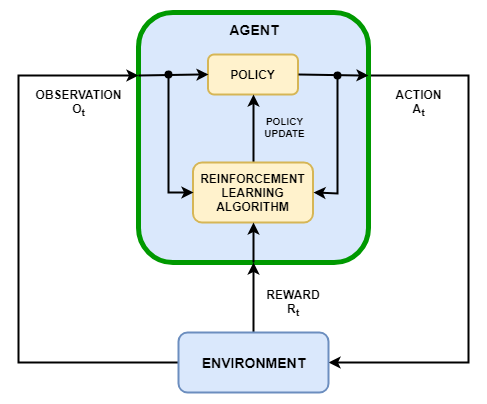
\includegraphics[width=\figwidth]{RL_architecture.png}
    \caption{強化學習架構}
    \label{fig:RL_architecture}
\end{figure}

\bigskip
% ---------- Modeling and training ----------
\section{建模與訓練}
\subsection{OpenAI GYM}

\bigskip
\subsection{訓練結果}

\bigskip
% ---------- Conclusion ----------
\section{結論}

\bigskip
% ---------- Refrence ----------
\titleformat{\section}{\bfseries\texttwelve}{\xCJKnumber{\thesection}、}{0em}{}
\printbibliography[title=\texttwelve{參考文獻}]

\end{multicols*}
\end{document}